%%==================================================
%% chapter02.tex for BIT Master Thesis
%% modified by yang yating
%% version: 0.1
%% last update: Dec 25th, 2016
%%==================================================
\chapter{背景及相关工作}
\label{chap:backinfo}

%本章主要介绍,关于……的背景
本章的主要内容,是介绍关于VoLTE及时间隐通道的相关背景,并对国内外的研究现状进行分析阐述。本章首先分析了VoLTE音视频传输方案,研究在VoLTE中构建时间隐通道的可行途径。接下来分析了现有的时间隐通道构建方案,研究时间隐通道构建方法中需要注意的关键点。然后分析VoLTE传输协议,研究构建方法的依赖元素。进一步分析现有的时间隐通道检测方法,研究不同方法的特点及适用范围。最后总结时间隐通道的构建指标,列举了时间隐通道应当满足的要求。

%及国内外相关工作的概述

%在下方加入各小节内容
\section{VoLTE音视频传输方案}
\label{chap:backinfo:volte}

%VoLTE实现概述

\insertFigure{
	\begin{figure}[htbp]
		\centering
        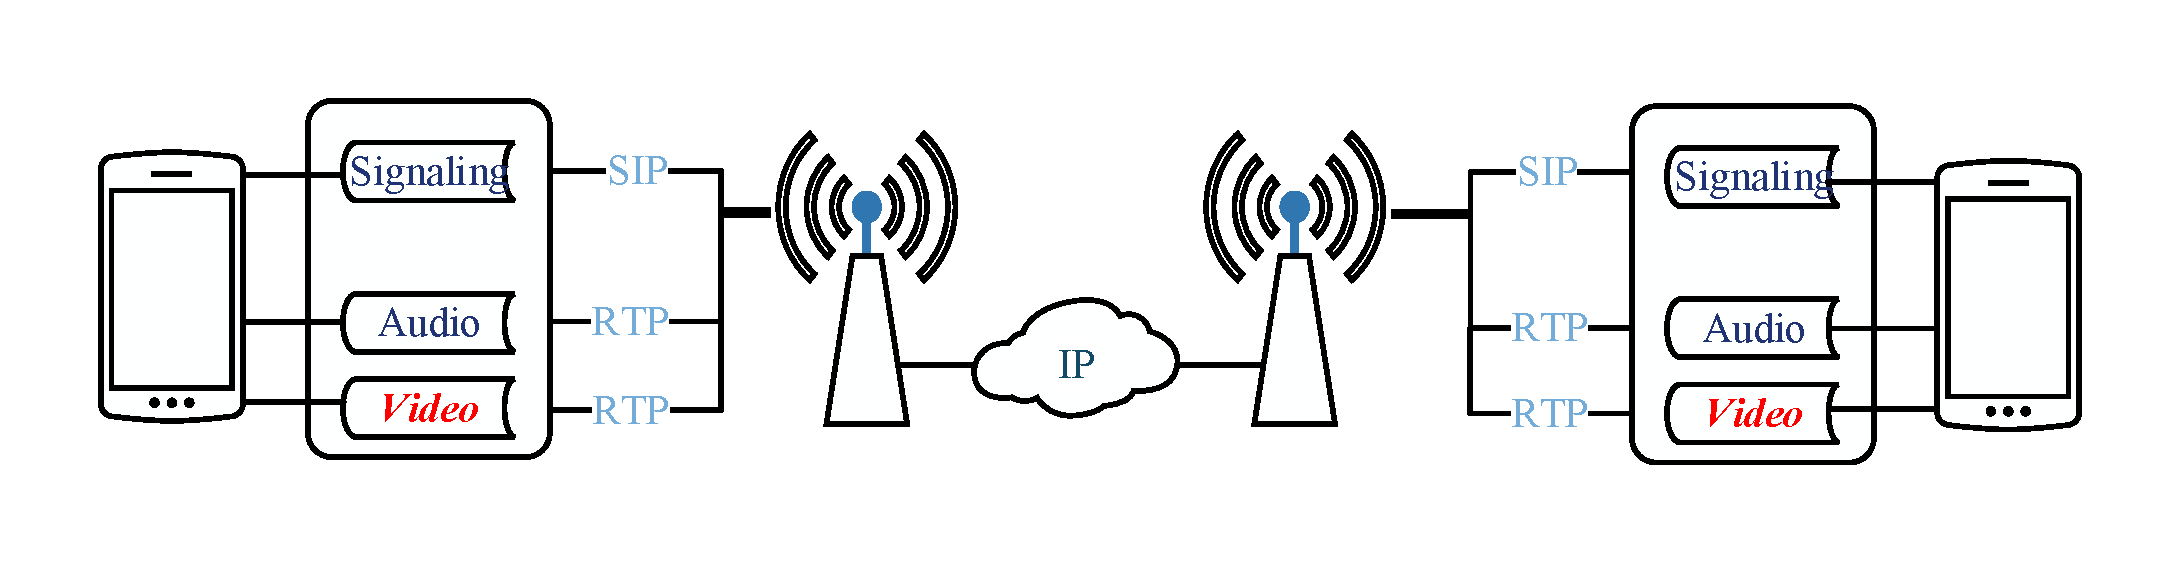
\includegraphics[width=0.95\textwidth]{chapters/chapter2/figures/volte-model.pdf}
        \caption{VoLTE视频通话中的数据流}\label{fig:2:volte-model}
	\end{figure}
}

语音通信功能是移动通信技术的基本需求,随着智能终端的发展,用户的移动数据需求才逐渐占据主流。在移动通信标准中,基于LTE的第四代移动通信技术已经转变为全IP网络,实现了语音主导到数据主导的转换。不同于原有的通信方案,LTE对数据传输进行了优化,同时对音视频通话功能进行了升级。

\subsection{VoLTE数据处理流程}
\label{chap:backinfo:volte:datastream}

在2G及3G时代,基于电路交换音频通话技术,是支撑语音业务的核心解决方案。进入4G时代,核心网络改变为全数据包交换,基于电路交换的音频通话已经无法兼容,需要全新的通话模式。于是,类似于VoIP音视频解决方案,基于LTE的VoLTE成为4G时代的音视频通话方案。在实际应用中,支持VoLTE的终端能够快速建立呼叫,否则将回落到3G或2G网络,从而兼容多种设备及场景。\nupcite{poikselka2012voice}

如图\nref{fig:2:volte-model},VoLTE视频通话过程中,需要三个数据信道,分别为信令信道、语音信道及视频信道,所有的信道均采用数据包进行传输。通过音视频分离方式,VoLTE实现了多场景兼容。通过信令信道,对通话模式及参数进行协商,决定语音信道及视频信道采用的编码方式。相对2G及3G网络,LTE支持的数据上行速率有了显著提升,能够支撑更多的终端进行高清晰度通话。\nupcite{ZHANG201929}

\insertTable{
    \begin{table}[htbp]
        \centering
        \caption{LTE业务QCI分配表概述}
        \label{tab:2:qci-classification}
        \begin{threeparttable}
            \begin{tabular*}{\textwidth}{@{\extracolsep{\fill}}cccccc}
                \toprule
                QCI\tnote{1}分类 & 资源类型 & 优先级 & 可接受延迟 & 可接受丢包率 & 服务类型 \\ 
                \midrule
                1 & 保证QoS\tnote{2} & 2 & 100 ms & $10^{-2}$ & VoLTE语音 \\ 
                2 & 保证QoS & 4 & 150 ms & $10^{-3}$ & VoLTE视频 \\
                5 & 不保证QoS & 1 & 100 ms & $10^{-6}$ & VoLTE信令 \\
                7 & 不保证QoS & 7 & 100 ms & $10^{-6}$ & 交互式音视频应用 \\
                \bottomrule
            \end{tabular*}
            \begin{tablenotes}
                \footnotesize
                \item[1] QCI指Quality of Service Class Identifiers,QoS分类标签
                \item[2] QoS指Quality of Service,服务质量
            \end{tablenotes}
        \end{threeparttable}
    \end{table}
}

相较于固网,移动无线网络受噪声干扰明显,导致用户通话体验变差。如表\nref{tab:2:qci-classification},根据LTE业务分类,VoLTE的信令数据包具有1级最高优先级,可接受时延为{100\ ms},可接受丢包率为$10^{-6}$;VoLTE语音数据包具有2级优先级,可接受时延为{100\ ms},可接受丢包率为$10^{-2}$;VoLTE视频数据包优先级降为4级,可接受时延为{150\ ms},可接受丢包率为$10^{-3}$。另一方面,即使VoIP应用的数据包也是经LTE网络传输,其服务质量也是完全不同的,运营商网络只保证尽力传输。VoIP应用的音视频数据对应的优先级为7,可接受时延为{100\ ms},可接受丢包率为$10^{-6}$。\nupcite{7154042,6996582,Li:2015:IVS:2810103.2813618}

因此,VoLTE相较于其它VoIP应用,受网络调度产生抖动的几率要小。时间隐通道的操作空间较小,对构建方法提出了新的挑战。

\subsection{VoLTE数据包传输特征}
\label{chap:backinfo:volte:packets}
%VoLTE音视频分流处理的模式(分清楚执行组件),结合传输的逻辑设计
通过支持VoLTE的终端设备进行视频通话,参与数据处理的处理器通常由两部分组成。其中一个是AP(Application Processor)也就是应用处理器,另外一个是BP(Baseband Processor)也就是基带处理器。AP参与操作系统中通用数据的处理,BP负责的是无线通信数据的处理,二者相互补充,共同完成智能终端设备的数据处理任务。

\insertFigure{
	\begin{figure}[htbp]
		\centering
        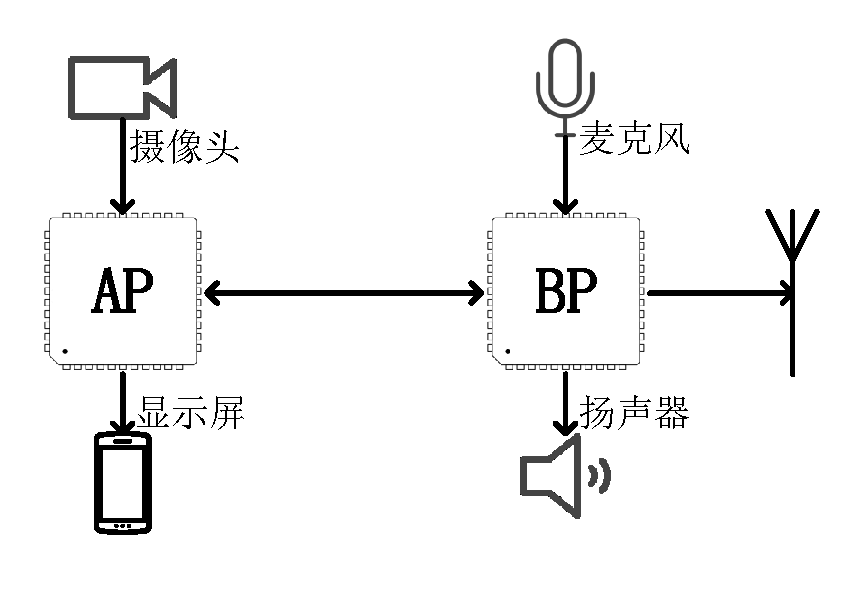
\includegraphics[width=0.55\textwidth]{chapters/chapter2/figures/ap-bp.pdf}
        \caption{VoLTE视频通话时AP与BP功能划分}\label{fig:2:ap-bp}
	\end{figure}
}

如图\nref{fig:2:ap-bp},AP与BP对应不同的媒体类型。对于VoLTE语音数据,由基带处理器按照设定的时间间隔,完成模拟信号的采样、编码,并将打包好的语音数据包通过射频系统传输。对于VoLTE视频数据,由于图像处理模块集成在应用处理器中,视频数据包需要应用处理器参与。应用处理器调用摄像系统驱动,获取编码后的视频数据流,按照视频帧分别进行切片打包,得到RTP视频数据包。视频数据包由系统内核中的协议栈发送,最终由BP通过射频系统传输。类似的,在接收阶段,VoLTE语音数据由基带处理器完成接收、解包、解码,并交由扬声器进行播放。VoLTE视频数据包则交付系统中的网络组件,完成解包、解码后,由通话软件显示在屏幕上。\nupcite{ZHANG201929,guo2019volte}

%抓包结果,分析传输特征,时间间隔、发送密度
\subsubsection{音视频数据包发送特征}
\label{chap:backinfo:volte:packets:send}

\insertFigure{
    \begin{figure}[htbp]
        \centering
        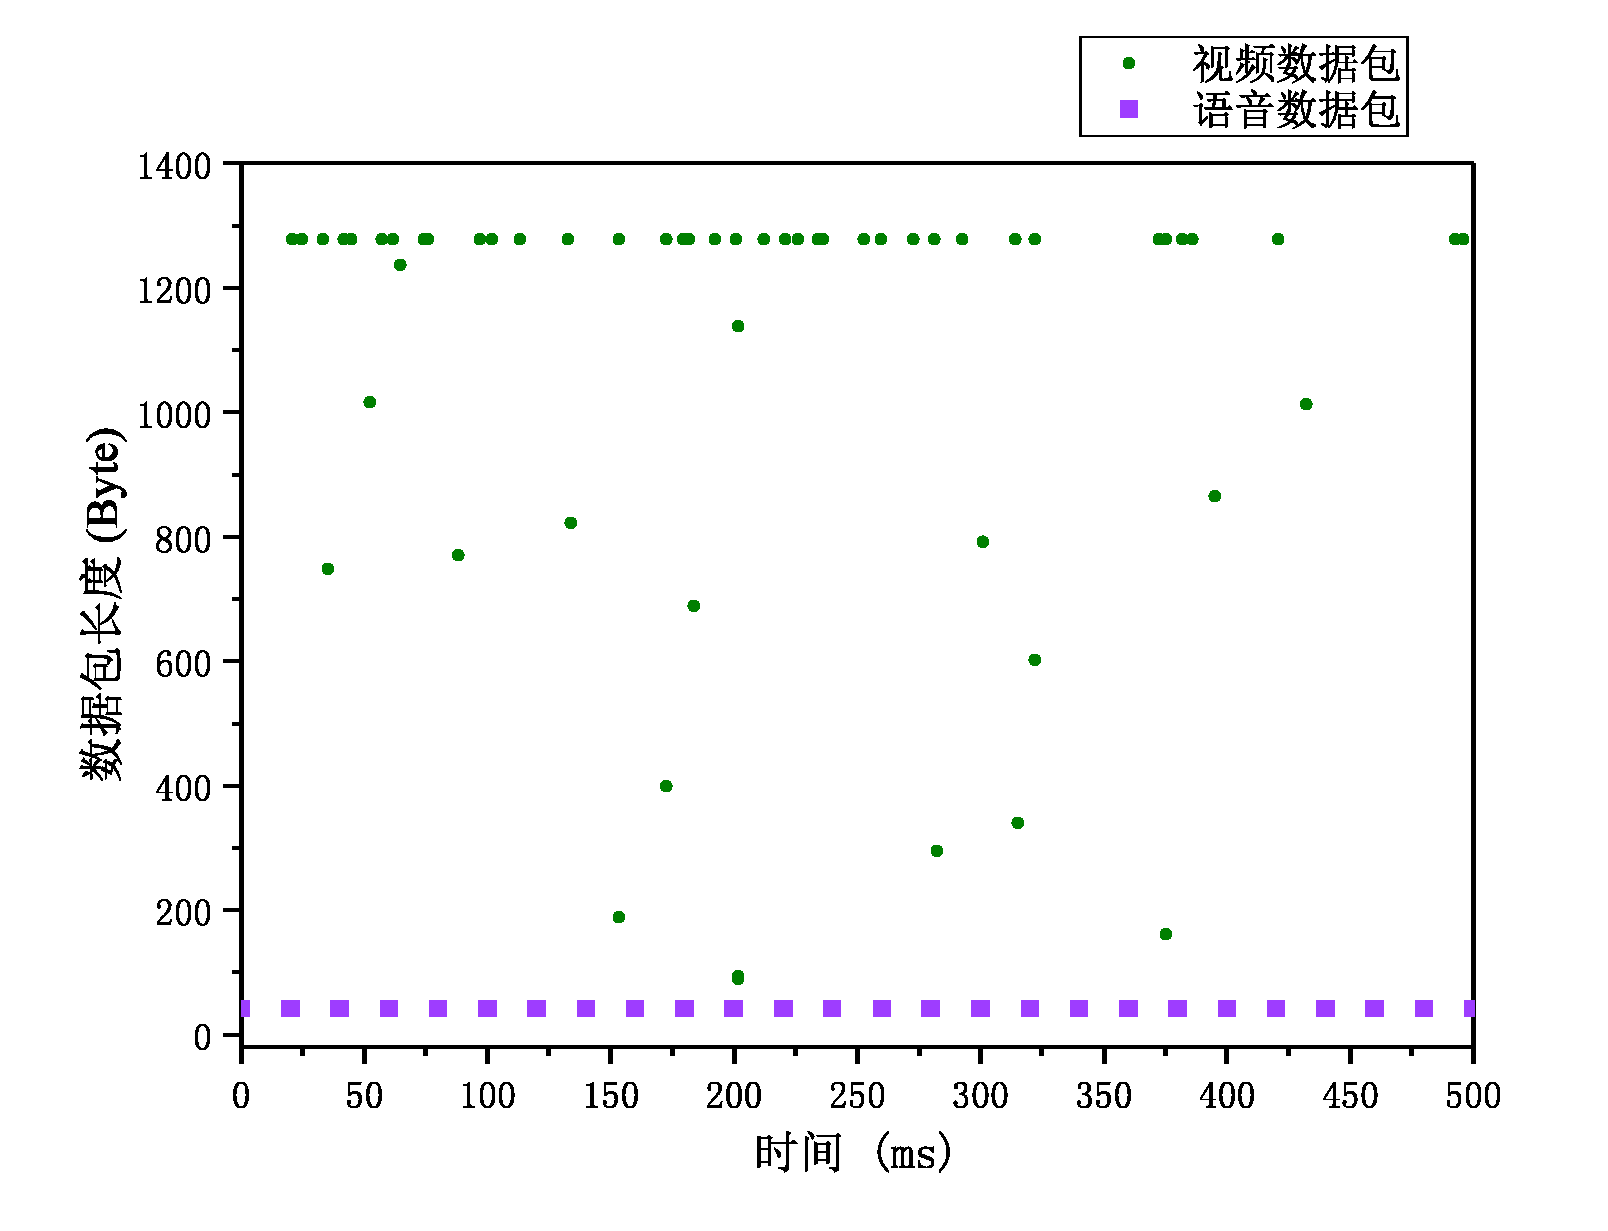
\includegraphics[width=0.75\textwidth]{chapters/chapter2/figures/length-audio-video.pdf}
        \caption{VoLTE音视频数据包发送间隔示意}\label{fig:2:audio-video}
    \end{figure}
}

对于音频数据包,采用AMR-WB(Adaptive Multi-Rate Wideband)格式编码时,数据包在非静音期每{20\ ms}发送一次,在静音期不发送数据包。\nupcite{8288828}对于视频数据包,数据包发送间隔取决于视频刷新率及编码结果,具有很大的不确定性。\nupcite{zhang2019timestamp}如图\nref{fig:2:audio-video},VoLTE视频数据包的长度虽然在{1300\ 字节}左右有集中分布,但仍有部分数据包长度随机变化;另一方面,VoLTE语音数据包的发送间隔具有规律性,相比较视频数据包的聚集现象更普遍。

\subsubsection{视频数据包发送与接收IPD分布特征}
\label{chap:backinfo:volte:packets:ipd}
如本文\nref{chap:backinfo:volte:packets:send}所述,VoLTE语音数据包的IPD规律性明显,对构建时间隐通道不利。研究VoLTE视频数据包的传输特征,对VoLTE下时间隐通道构造方法的研究具有重要意义,VoLTE视频数据流对噪声敏感度低,便于时间隐通道隐匿在网络噪声中。

\insertFigure{
    \begin{figure}[htbp]
        \centering
        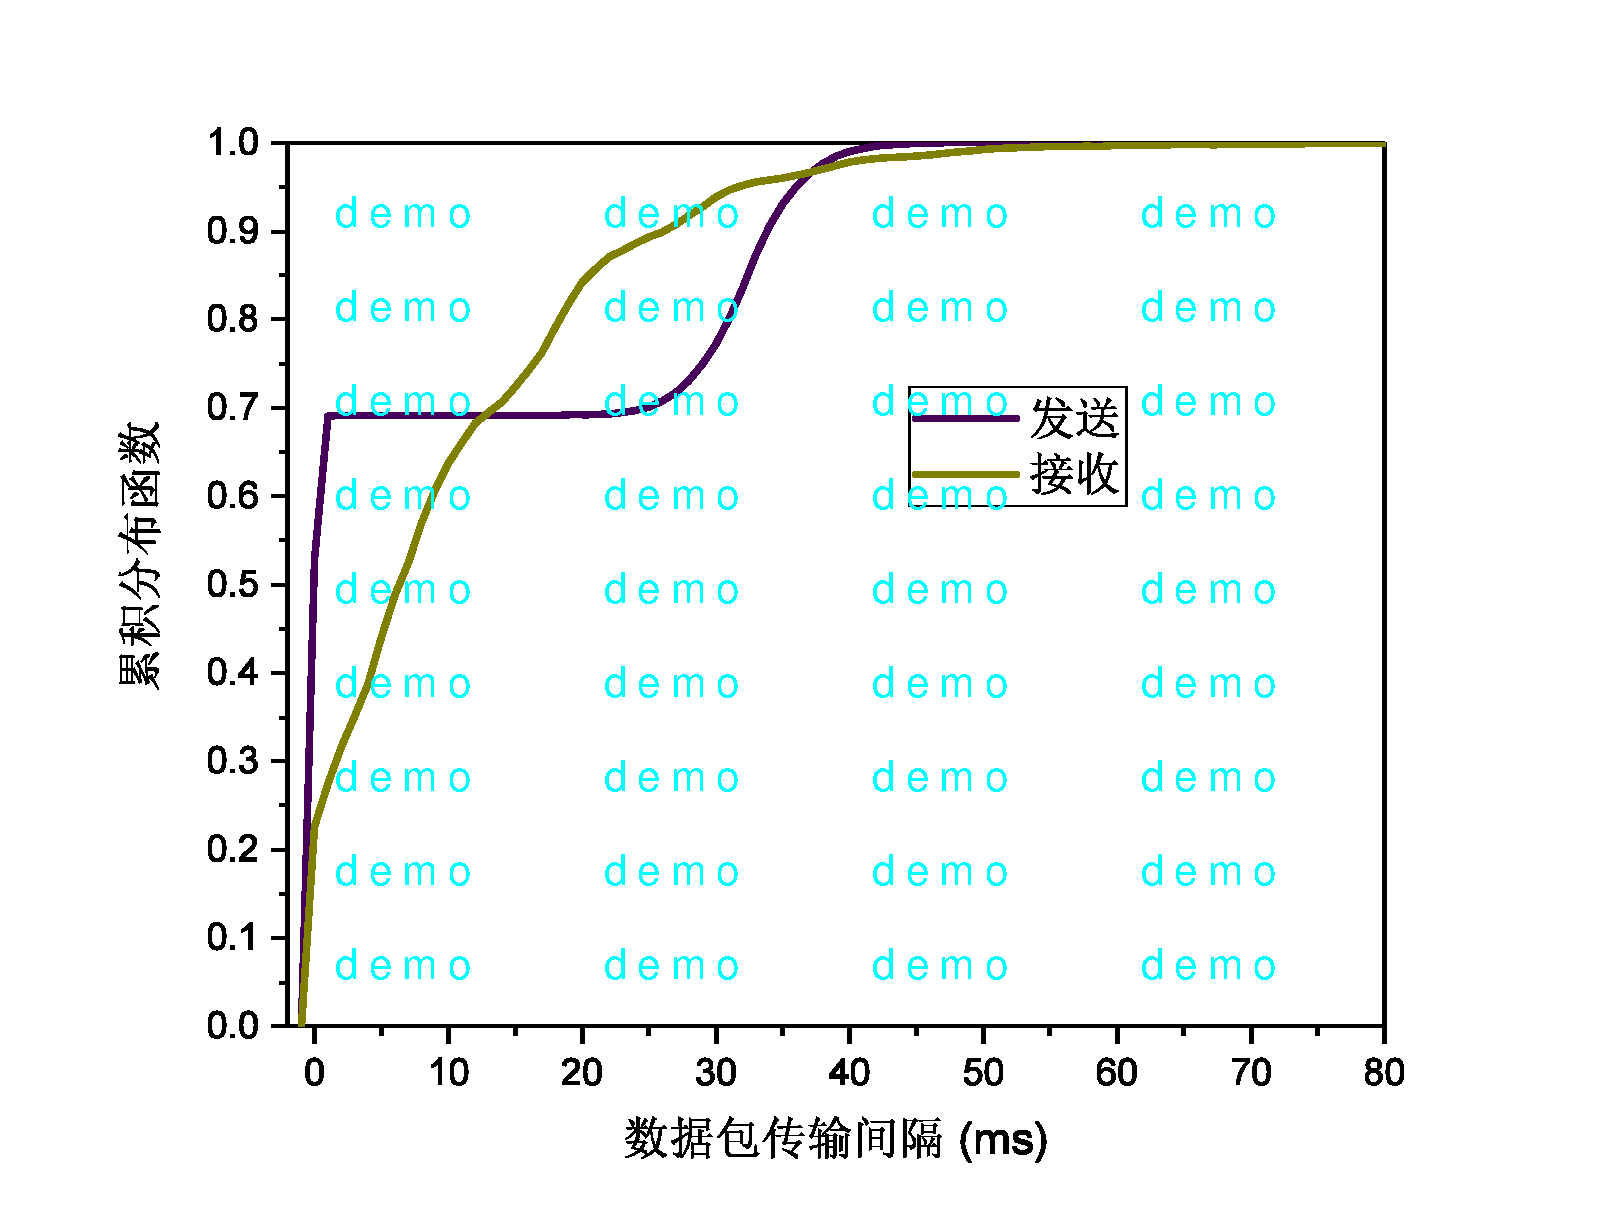
\includegraphics[width=0.7\textwidth]{chapters/chapter2/figures/cdf-send-receive.pdf}
        \caption{VoLTE视频数据包IPD的累积分布函数}\label{fig:2:cdf-ipd}
    \end{figure}
}

如图\nref{fig:2:cdf-ipd},在发送阶段,IPD主要集中在{30\ ms}及{0\ ms}两部分,由于视频刷新率为{30\ fps},每隔{33\ ms}产生一个新的视频帧,而视频帧又有多个数据包组成,造成发送阶段CDF曲线不平滑。在接收阶段,受网络噪声及传输延迟的影响,IPD在$[0,\ 30]$区间内集中分布,CDF曲线趋于平滑。因此,视频数据包在IPD方面,对时间隐通道的容忍性要优于语音数据包。

\subsubsection{VoLTE视频数据包丢包特征}
\label{chap:backinfo:volte:packets:dropout}

\insertFigure{
    \begin{figure}[htbp]
        \centering
        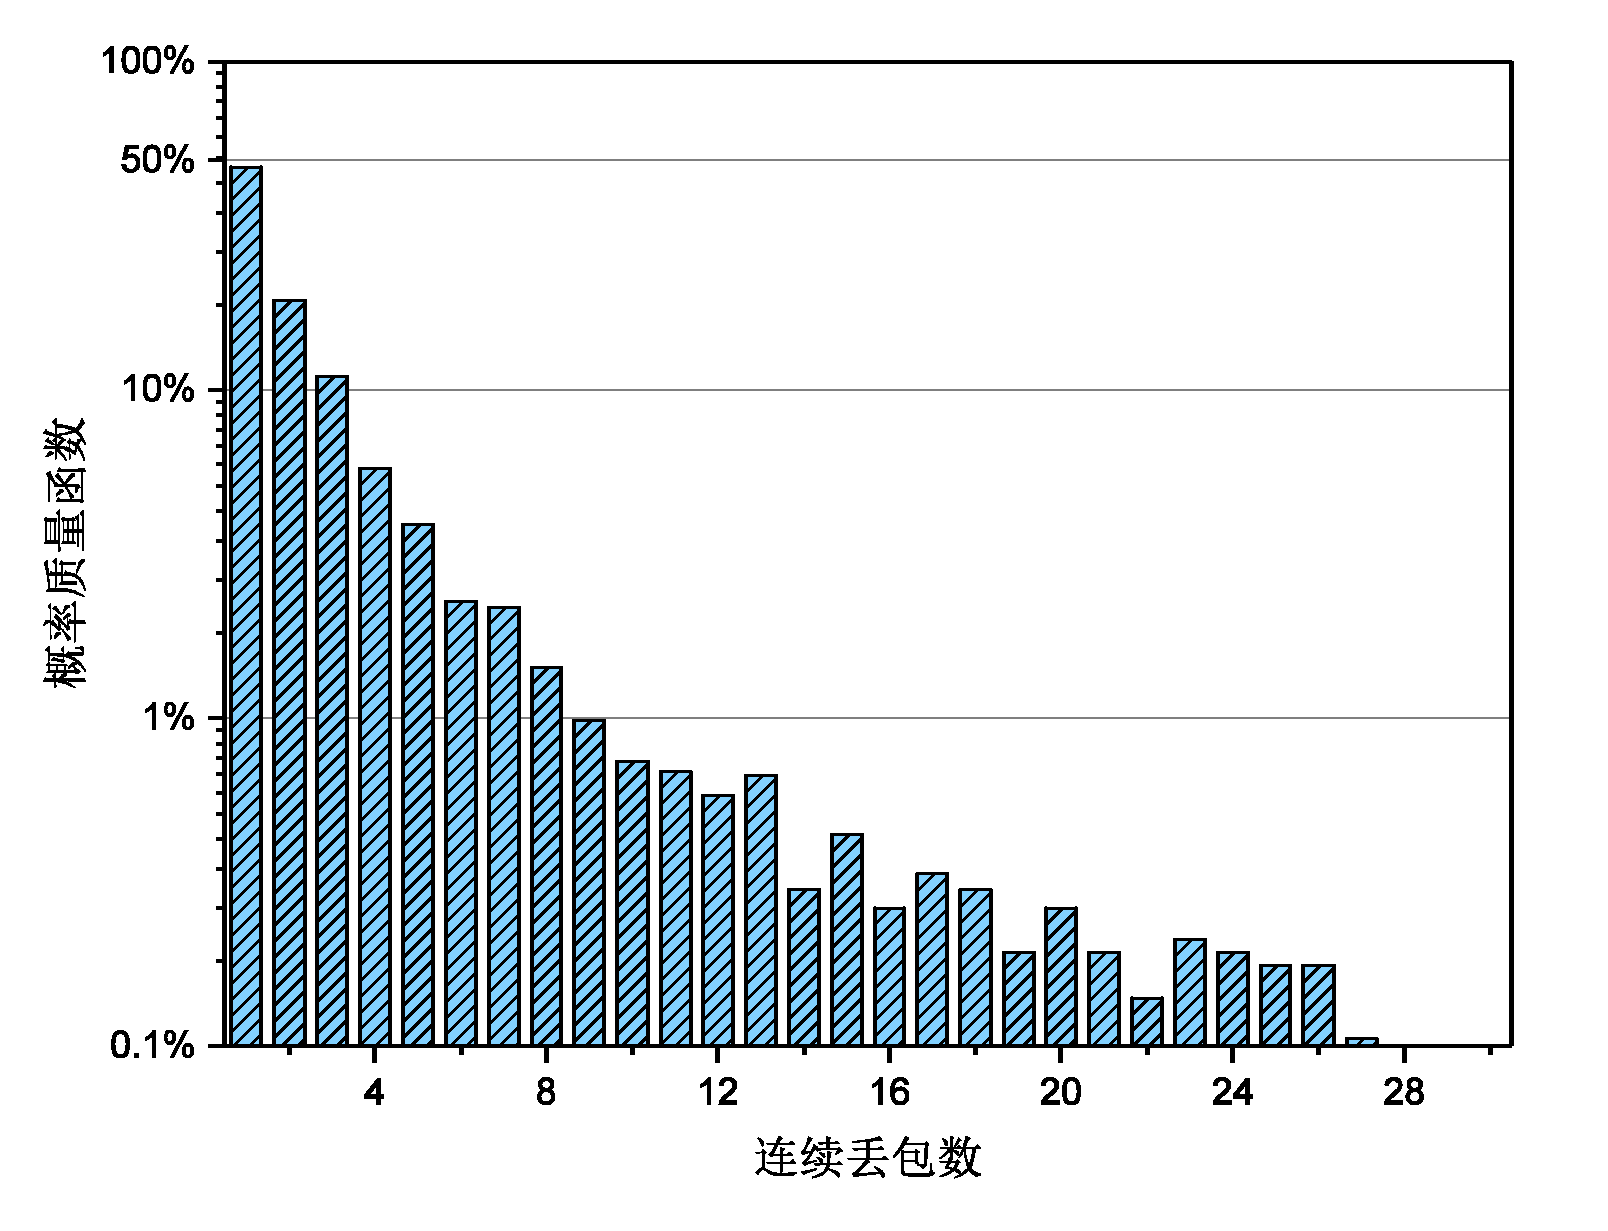
\includegraphics[width=0.7\textwidth]{chapters/chapter2/figures/pmf-dropout.pdf}
        \caption{连续丢包数量的概率质量函数}\label{fig:2:pmf-dropout}
    \end{figure}
}

对于VoLTE视频数据包,连续丢包数量的概率质量函数如图\nref{fig:2:pmf-dropout}。该统计结果,来自抓包得到的58万条VoLTE视频数据包,包含低噪声及高噪声在内的多种测试场景。PMF(Probability Mass Function)统计结果显示,VoLTE视频数据信道中的丢包事件,主要由单个离散丢包事件组成,连续大量的丢包事件占据的比例非常小。

\subsection{基于主动丢包的时间隐通道构建基础}
\label{chap:backinfo:volte:scheme}
VoLTE出现丢包的原因,主要由于通信终端与基站的空口传输过程。在复杂的无线环境中,发送端与接收端均会出现丢包可能。对于监听者,只有监听了隐通道发送方的终端设备,才有一定几率发现机遇主动丢包的时间隐通道。然而,在隐通道的威胁模型及实际应用中,监听者主要监听的是中间介质,基于主动丢包的时间隐通道,符合VoLTE的传输特征。

通过对VoLTE通话的理论及实际分析测试,在VoLTE场景中构建时间隐通道,尤其是通过主动丢包的方式构建时间隐通道,应当首先选择VoLTE视频信道作为宿主信道。与此同时,主动丢包的构建方式应当模拟离散丢包模式,并且在统计特征方面拟合已知统计结果。另一方面,VoLTE视频信道自身的丢包率,已经超过了QCI的预期丢包率,证明当前VoLTE仍然不能完全保证服务质量,通过主动丢包构建时间隐通道可行。所以,本文选择VoLTE视频信道,作为时间隐通道的宿主信道。 %VoLTE
\section{VoLTE音视频传输方案}
\label{chap:backinfo:volte}

%VoLTE实现概述

\insertFigure{
	\begin{figure}[htbp]
		\centering
        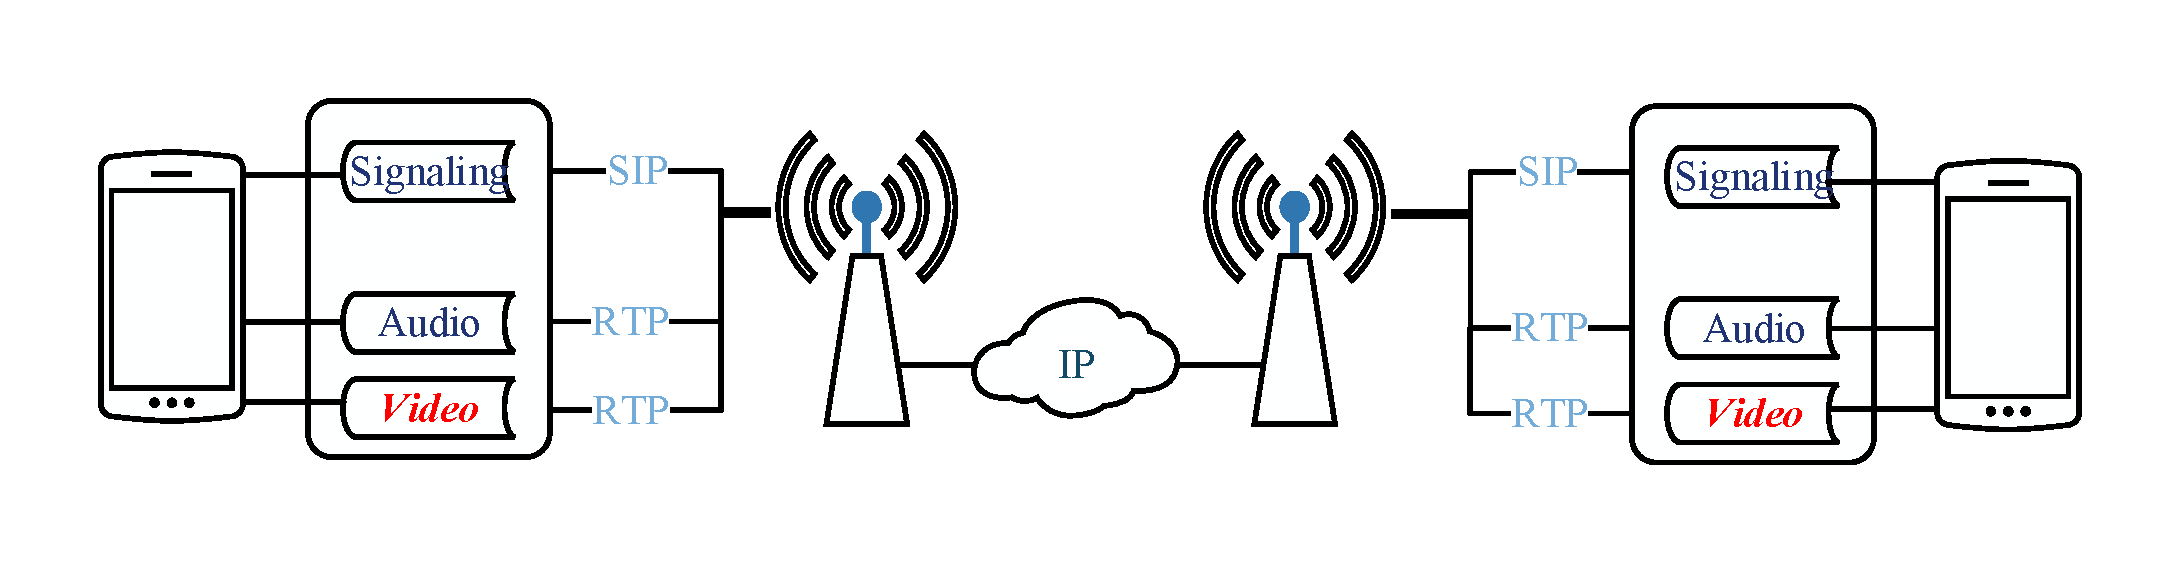
\includegraphics[width=0.95\textwidth]{chapters/chapter2/figures/volte-model.pdf}
        \caption{VoLTE视频通话中的数据流}\label{fig:2:volte-model}
	\end{figure}
}

语音通信是移动通信技术的基本需求,随着智能终端的发展,移动数据需求超过了语音通信需求。为满足用户移动宽带业务需求,基于LTE的第四代移动通信技术采用了全IP网络,实现了语音主导到数据主导的转换。新的传输模式下,LTE对数据传输进行了优化,同时提升了音视频通话业务能力。

\subsection{VoLTE数据处理流程}
\label{chap:backinfo:volte:datastream}

2G及3G时代,基于电路交换的音频通话技术,是支撑语音业务的核心解决方案。进入4G时代,核心网络已经转变为全数据包交换,基于电路交换的音频通话已经无法完全兼容,需要全新的解决方案。于是,类似VoIP音视频通话,基于LTE的VoLTE成为4G时代的音视频通话解决方案。实际应用中,支持VoLTE的终端能够快速建立呼叫,并且支持回落到3G或2G网络,从而兼容多种设备及场景\nupcite{poikselka2012voice, 8315208}。

如图\ \nref{fig:2:volte-model},VoLTE视频通话中,存在三个数据信道,分别为信令信道、语音信道及视频信道,所有的信道均通过数据包传输。采用音视频分离设计,VoLTE兼容了多种通话场景。通过信令信道协商通话模式及参数,决定语音信道及视频信道采用的编码方式。相较2G及3G网络,LTE数据上行速率得到提升,能够支撑更多的终端进行高清晰度通话\nupcite{ZHANG201929}。

\insertTable{
    \begin{table}[htbp]
        \centering
        \caption{LTE业务QCI分配表概述}
        \label{tab:2:qci-classification}
        \begin{threeparttable}
            \begin{tabular*}{\textwidth}{@{\extracolsep{\fill}}cccccc}
                \toprule
                QCI\tnote{1}分类 & 承载要求 & 优先级 & 可接受延迟 & 可接受丢包率 & 服务对象 \\
                \midrule
                1 & 保证QoS\tnote{2} & 2 & 100 ms & $10^{-2}$ & VoLTE语音 \\
                2 & 保证QoS & 4 & 150 ms & $10^{-3}$ & VoLTE视频 \\
                5 & 不保证QoS & 1 & 100 ms & $10^{-6}$ & VoLTE信令 \\
                7 & 不保证QoS & 7 & 100 ms & $10^{-6}$ & 交互式音视频应用 \\
                \bottomrule
            \end{tabular*}
            \begin{tablenotes}
                \footnotesize
                \item[1] QCI指Quality of Service Class Identifiers,QoS分类标签
                \item[2] QoS指Quality of Service,服务质量
            \end{tablenotes}
        \end{threeparttable}
    \end{table}
}

相较于固网,移动无线网络的噪声干扰不可忽视,用户通话体验与噪声强度相关。如表\ \nref{tab:2:qci-classification},根据LTE业务分类,VoLTE信令数据包具有1级最高优先级,可接受时延为{100\ ms},可接受丢包率为$10^{-6}$;VoLTE语音数据包具有2级优先级,可接受时延为{100\ ms},可接受丢包率为$10^{-2}$;VoLTE视频数据包优先级降为4级,可接受时延为{150\ ms},可接受丢包率为$10^{-3}$\nupcite{8329138}。另一方面,即使VoIP应用的数据包经LTE网络传输,其服务质量也低于VoLTE,运营商网络只保证尽力传输。VoIP应用的音视频数据对应的优先级为7,可接受时延为{100\ ms},可接受丢包率为$10^{-6}$\nupcite{7154042,6996582,Li:2015:IVS:2810103.2813618}。

因此,VoLTE较其它VoIP应用,受网络调度产生抖动的几率要小,传输更加稳定。因此时间隐通道的操作空间较小,对构建方法提出了挑战。

\subsection{VoLTE数据包传输特征}
\label{chap:backinfo:volte:packets}
%VoLTE音视频分流处理的模式(分清楚执行组件),结合传输的逻辑设计
支持VoLTE的终端设备进行视频通话,参与通话的处理器通常由两部分组成。其中一个是AP(Application Processor)也就是应用处理器,另一个是BP(Baseband Processor)也就是基带处理器。AP执行操作系统的通用数据处理,BP负责无线通信数据处理,二者相互补充,共同完成智能终端的数据处理任务。

\insertFigure{
	\begin{figure}[htb]
		\centering
        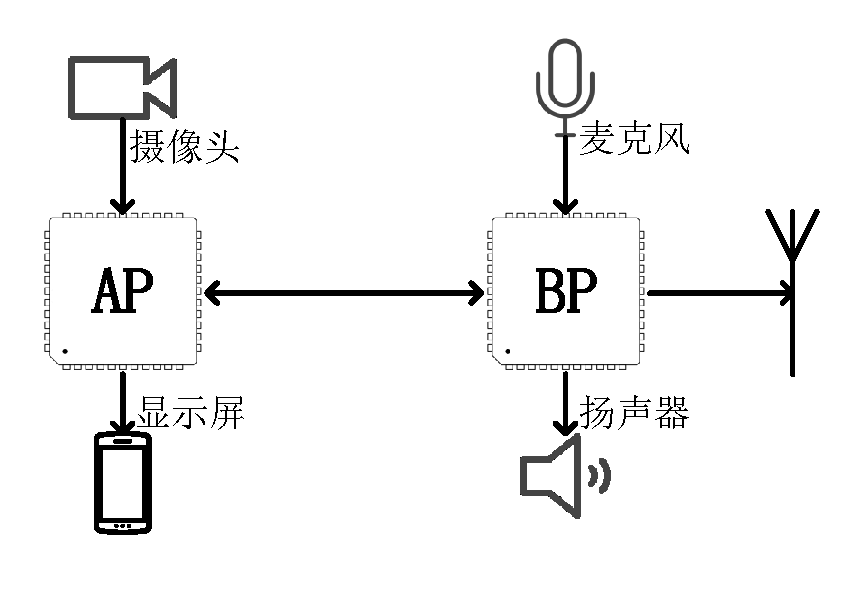
\includegraphics[width=0.55\textwidth]{chapters/chapter2/figures/ap-bp.pdf}
        \caption{VoLTE视频通话时AP与BP的功能划分}\label{fig:2:ap-bp}
	\end{figure}
}

如图\ \nref{fig:2:ap-bp},AP与BP处理不同的媒体类型。对于VoLTE语音数据,由基带处理器按照设定的时间间隔,完成模拟信号的采样、编码,并将打包好的语音数据包通过射频系统传输。对于VoLTE视频数据,由于图像处理模块集成在应用处理器中,视频数据需要应用处理器参与处理。应用处理器调用摄像系统驱动,获取编码后的视频数据,并以视频帧为单位进行打包,得到RTP视频数据包。视频数据包由系统内核中的协议栈发送,最终由BP通过射频系统传输。类似的,在接收阶段,VoLTE语音数据由基带处理器完成接收、解包、解码,并交由扬声器播放。VoLTE视频数据包则交付系统中的网络组件,完成解包、解码后,由通话软件显示在屏幕上\nupcite{ZHANG201929,guo2019volte}。

%抓包结果,分析传输特征,时间间隔、发送密度
\subsubsection{音视频数据包发送特征}
\label{chap:backinfo:volte:packets:send}

\insertFigure{
    \begin{figure}[htb]
        \centering
        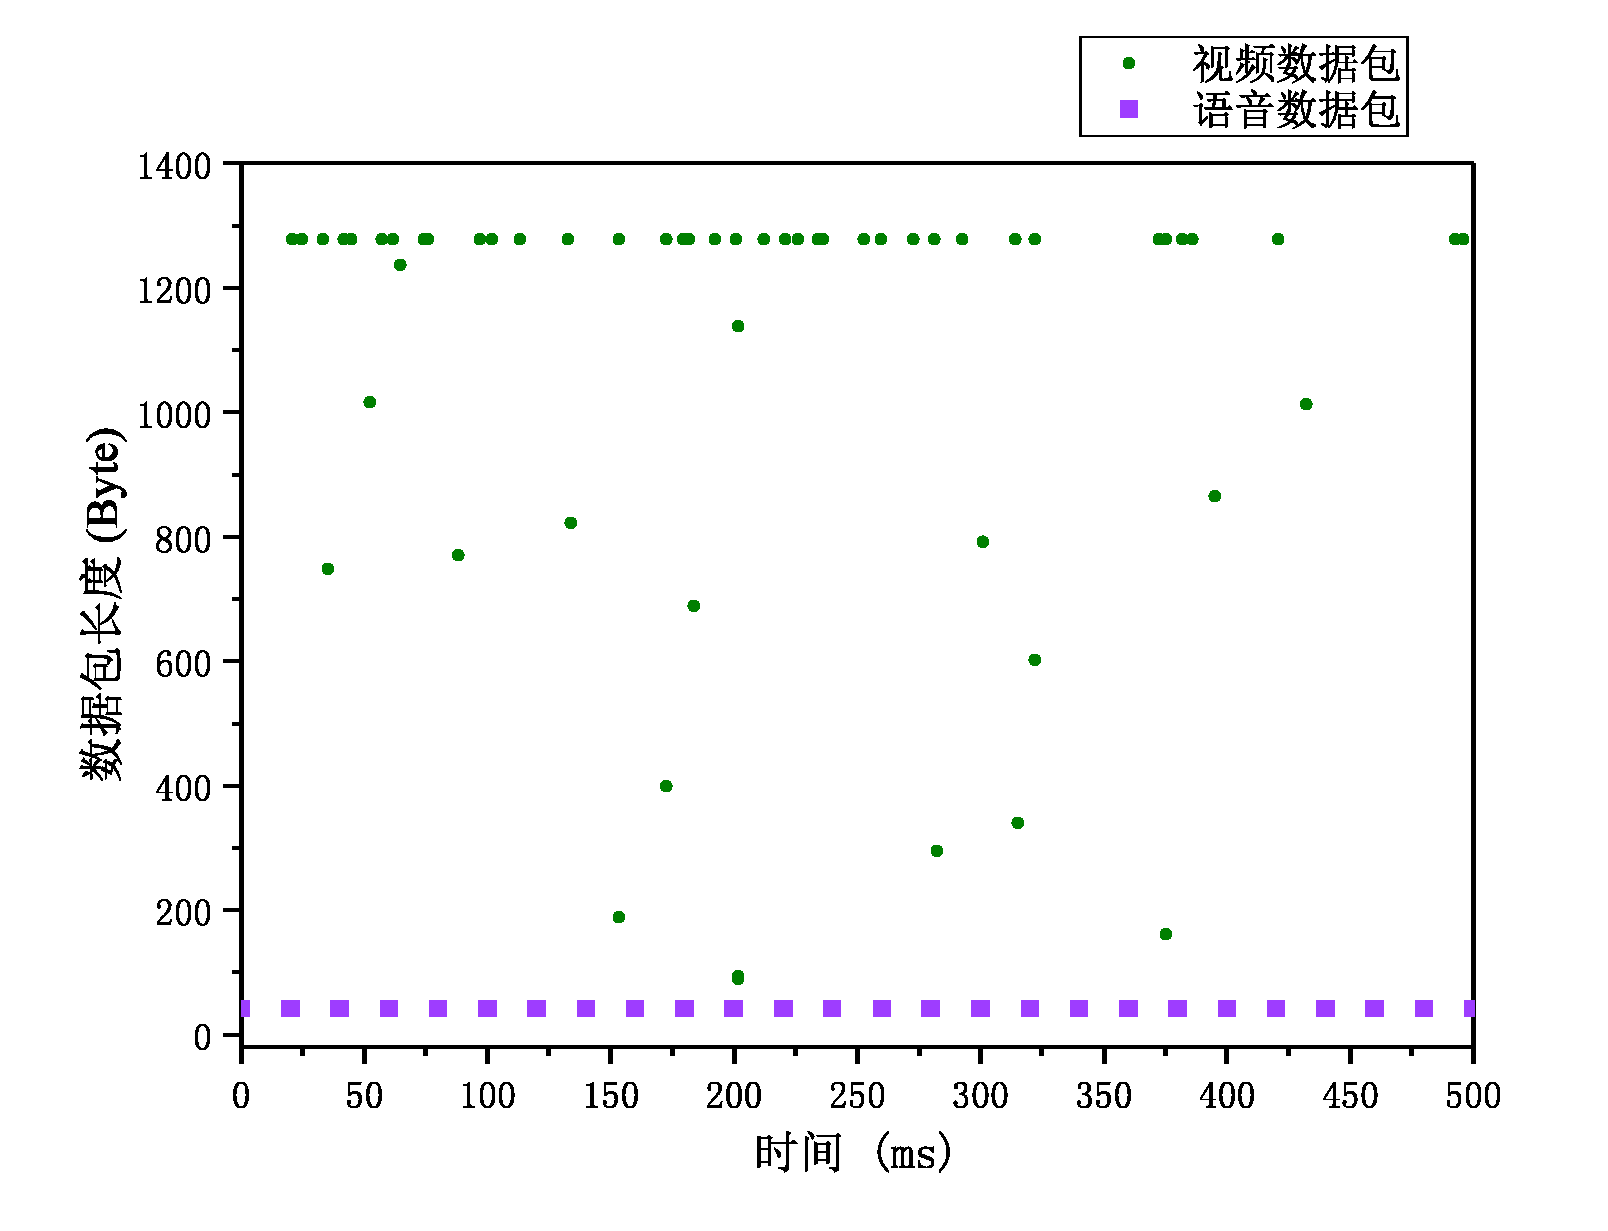
\includegraphics[width=0.75\textwidth]{chapters/chapter2/figures/length-audio-video.pdf}
        \caption{VoLTE音视频数据包发送间隔示意}\label{fig:2:audio-video}
    \end{figure}
}

对于音频数据包,采用AMR-WB格式编码时,非静音期每{20\ ms}发送一次数据包,静音期不发送数据包\nupcite{8288828}。对于视频数据包,数据包发送间隔取决于视频刷新率及编码结果,具有不确定性\nupcite{zhang2019timestamp}。如图\ \nref{fig:2:audio-video},虽然VoLTE视频数据包的长度多在{1300\ 字节}左右,但仍有部分数据包的长度随机变化;另一方面,VoLTE语音数据包的发送间隔具有规律性,而视频数据包多为密集发送。

\subsubsection{视频数据包IPD分布特征}
\label{chap:backinfo:volte:packets:ipd}
如本文\ \nref{chap:backinfo:volte:packets:send}所述,VoLTE语音数据包的IPD存在规律,因此不利于构建时间隐通道。研究VoLTE视频数据包的传输特征,对VoLTE时间隐通道构建方法具有重要意义。

\insertFigure{
    \begin{figure}[htb]
        \centering
        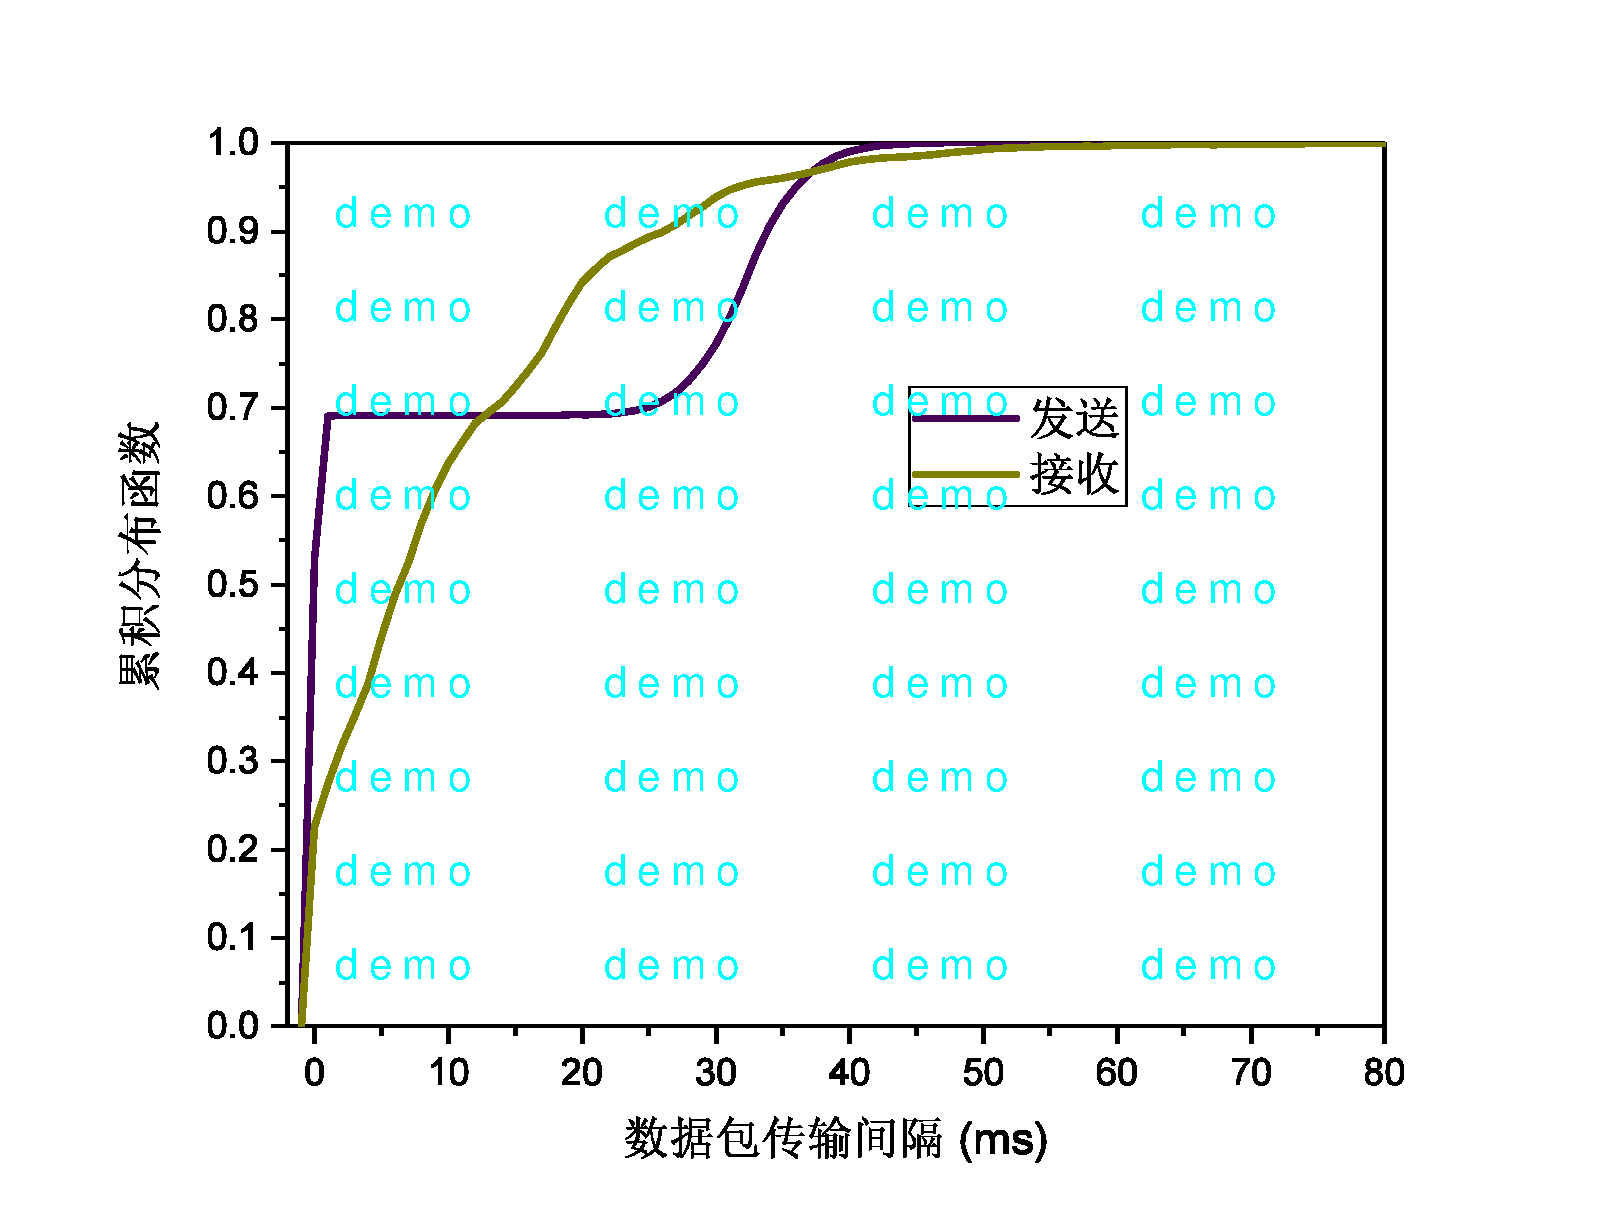
\includegraphics[width=0.7\textwidth]{chapters/chapter2/figures/cdf-send-receive.pdf}
        \caption{VoLTE视频数据包IPD的累积分布函数}\label{fig:2:cdf-ipd}
    \end{figure}
}

如图\ \nref{fig:2:cdf-ipd},发送阶段IPD主要集中在{30\ ms}及{0\ ms}。由于视频刷新率为{30\ fps},每隔{33\ ms}产生一个新的视频帧,而视频帧又由多个数据包组成,导致发送阶段CDF曲线不平滑。接收阶段,受网络噪声及传输延迟的影响,IPD集中在$[0,\ 30]$区间内,CDF曲线趋于平滑。因此在IPD方面,视频数据包对时间隐通道的容忍度高于语音数据包。

\subsubsection{VoLTE视频数据包丢包特征}
\label{chap:backinfo:volte:packets:dropout}

\insertFigure{
    \begin{figure}[htbp]
        \centering
        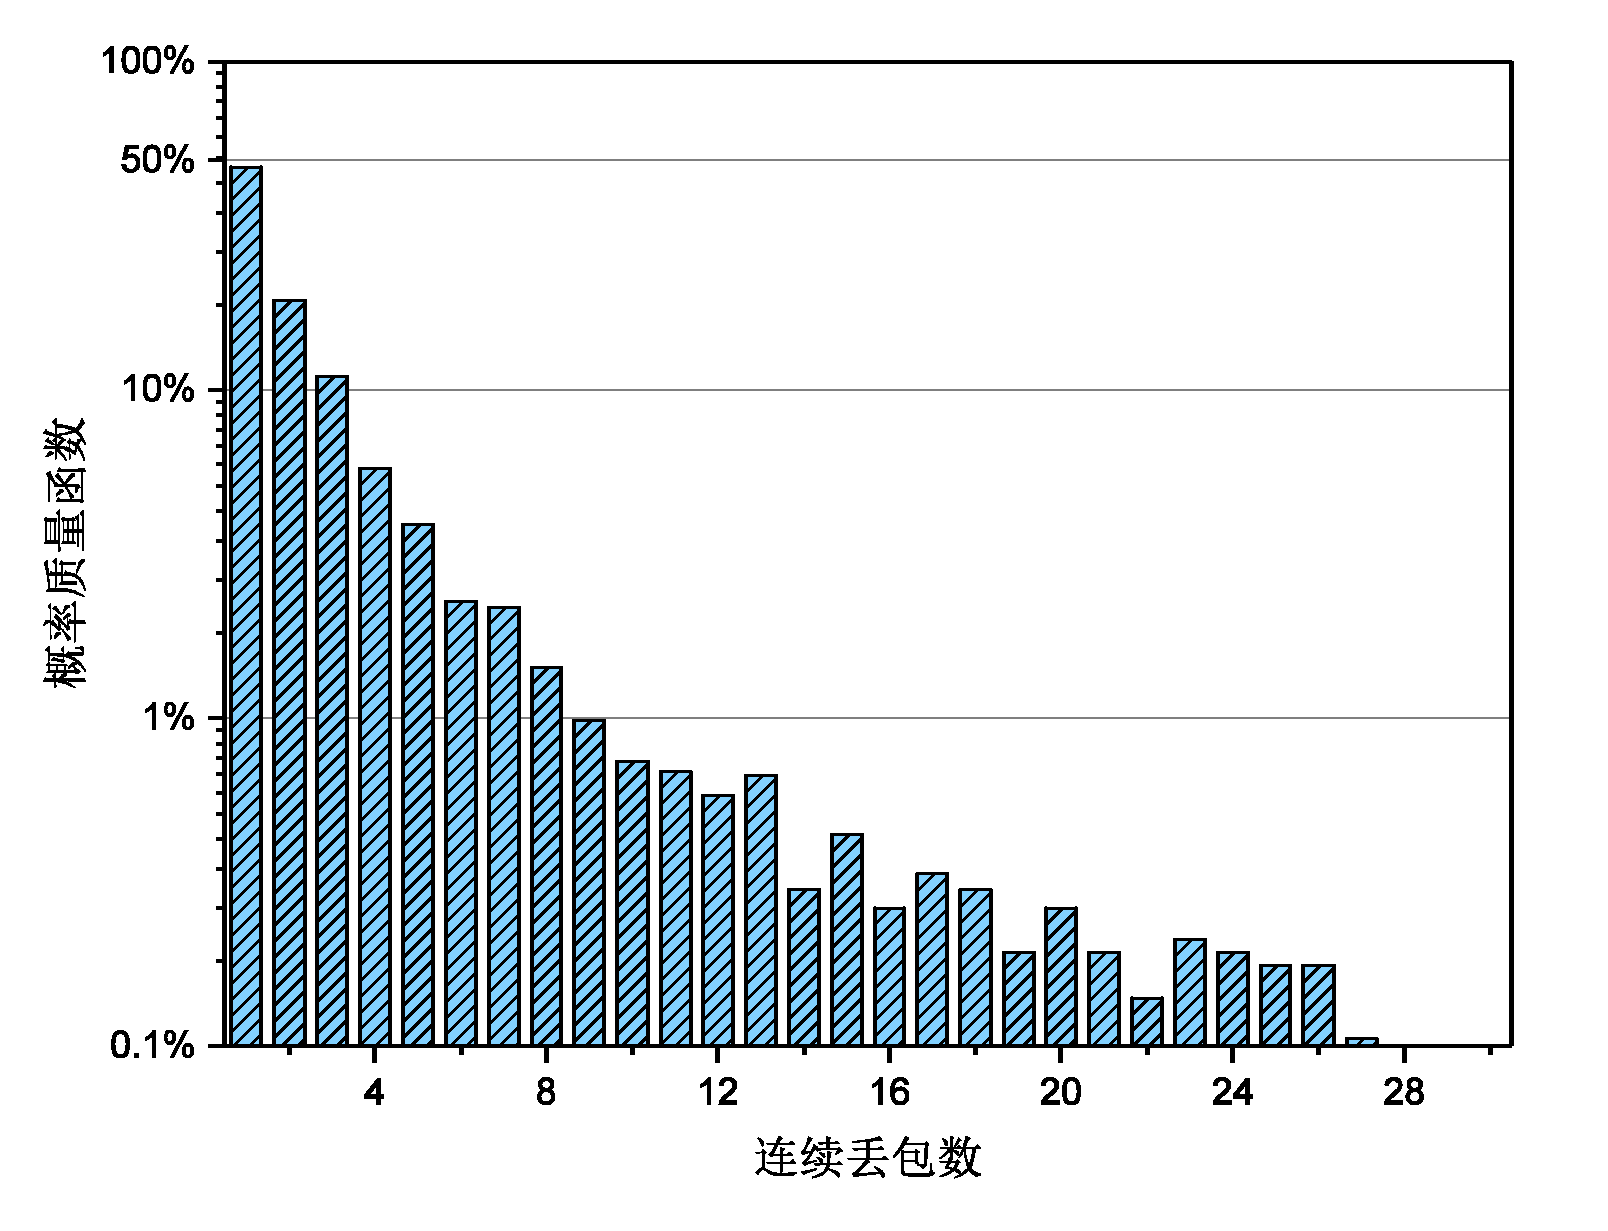
\includegraphics[width=0.7\textwidth]{chapters/chapter2/figures/pmf-dropout.pdf}
        \caption{连续丢包数的概率质量函数}\label{fig:2:pmf-dropout}
    \end{figure}
}

对于VoLTE视频数据包,连续丢包数的概率质量函数如图\ \nref{fig:2:pmf-dropout}。该统计结果,来自抓包得到的58万条VoLTE视频数据包,包含低噪声及高噪声在内的多种测试场景。PMF(Probability Mass Function)统计结果显示,VoLTE视频信道中的丢包事件,主要由单个离散丢包事件组成,连续丢包事件占据的比例较小。

\subsection{基于主动丢包的时间隐通道构建}
\label{chap:backinfo:volte:scheme}
VoLTE出现丢包的原因,主要是终端与基站空口传输过程的干扰。复杂的无线网络环境中,发送端与接收端均存在丢包可能性。对于监听者,只有监听了隐通道发送方的终端设备,才有一定几率发现基于主动丢包的时间隐通道。然而,在隐通道威胁模型及实际应用中,监听者主要监听中间媒介,因此基于主动丢包的时间隐通道,只需要保证统计特征方面的一致性即可。

通过对VoLTE通话的理论及数据分析,在VoLTE场景中构建时间隐通道,尤其是通过主动丢包的方式构建时间隐通道,应当选择VoLTE视频信道作为宿主信道。与此同时,主动丢包的结果应当模拟离散丢包模式,并且在统计特征方面拟合已知结果。另一方面,VoLTE视频信道的丢包率,已经超过了QCI的预期丢包率,表明当前LTE网络不能完全保证服务质量,通过主动丢包构建时间隐通道可行。 %CTC
\section{VoLTE传输协议分析}
\label{chap:backinfo:rtp}

VoLTE实在RTP协议的基础上实现的,RTP自身有一些特征

在这里进行的分析,如何利用这些特征,构造时间隐通道

\subsection{RTP数据包结构}
\label{chap:backinfo:rtp:struct}

RTP是怎样的标准,数据包等层次解析

RTP头的组成

\subsection{随机字段}
\label{chap:backinfo:random}

RTP参数中,包含哪些随机生成的字段

SSRC、TimeStamp,生成的效果

可以用于时间隐通道的秘钥及随机特征生成,保证保密性

\subsection{RTP丢包处理}
\label{chap:backinfo:dropout}

RTP及应用中,对于丢包事件的处理

丢包不重传,序号保证自增,是主动丢包方法的基础
 %RTP
\section{时间隐通道检测方法}
\label{chap:backinfo:detect}

%本节主要介绍,现有的时间隐通道检测方法,主要包括哪些
时间隐通道的发展,催生了新的时间隐通道检测技术。基于统计及分布一致性的时间隐通道检测方法,是常用的检测方法。某些场景中,基于标准差的检测方法,以及基于机器学习的检测方法也是有效的。\nupcite{ARCHIBALD2014284}

\subsection{基于分布曲线的检测}
\label{chap:backinfo:detect:statistical}

%统计看CDF差异,主要评估了哪些参数
传输过程中的时间特征,是时间隐通道检测方法的检测目标,基本的检测对象为IPD。当传输延迟恒定时,发送方观测到的IPD分布与接收方观测到的IPD分布是一致的。然而,存在网络噪声或者时间隐通道时,IPD分布出现偏离。时间隐通道检测方法,通过对比分布之间的最大偏离程度,从而判断是否存在隐通道。
\insertEquation{
    \begin{equation}
    \label{equ:2:ks}
		D_{KS}\ =\ sup_{x}\ |F_{1,\ n}(x)\ -\ G_{1,\ m}(x)|
    \end{equation}
    \begin{equation}
    \label{equ:2:ks-p}
        D_{KS,\ 0.05}\ =\ 1.358\ \times\ \sqrt{\frac{n\ +\ m}{n\ \times\ m}}
    \end{equation}
}
\insertFigure{
	\begin{figure}[htbp]
		\centering
        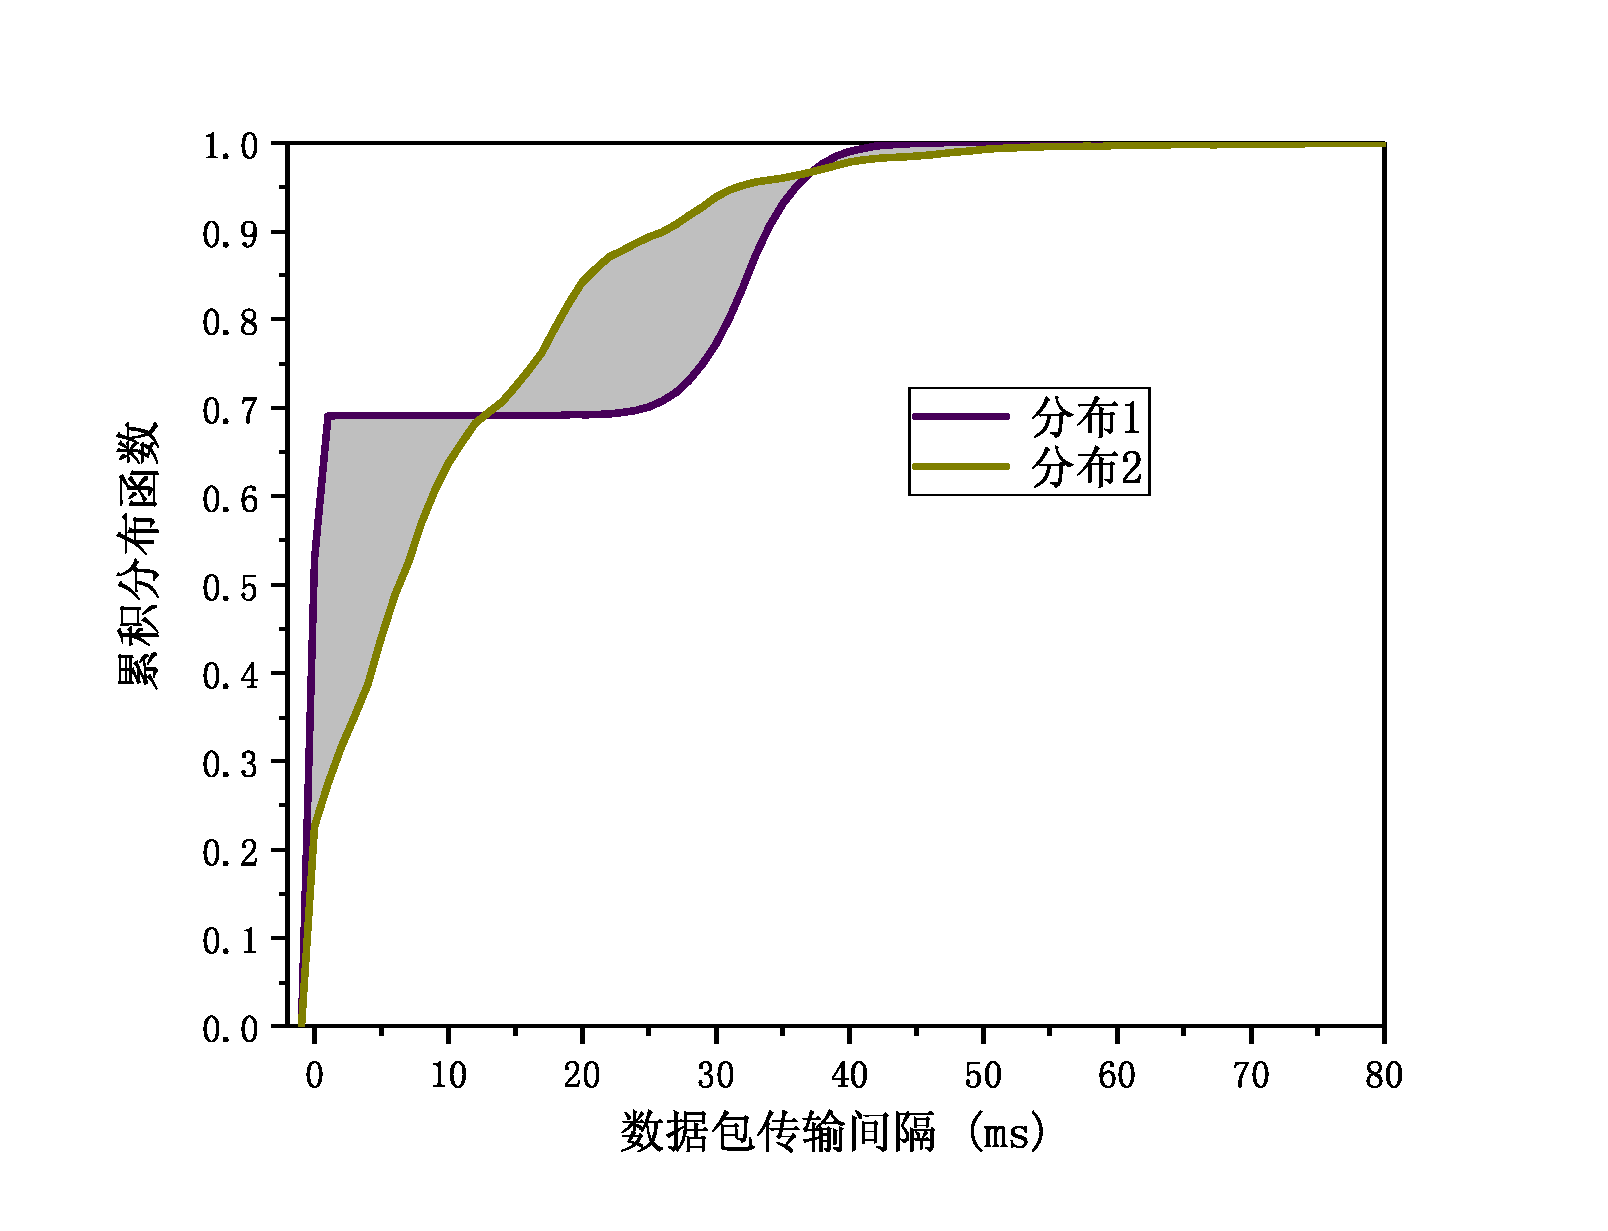
\includegraphics[width=0.7\textwidth]{chapters/chapter2/figures/ks-cdf.pdf}
        \caption{CDF曲线差异示意图}\label{fig:2:ks-cdf}
	\end{figure}
}

%如何根据差异,判断一致性
如图\nref{fig:2:ks-cdf},不同的CDF曲线代表不同的IPD分布。通过公式(\nref{equ:2:ks}),计算CDF曲线差异绝对值的最大值,得到分布曲线之间的直接差异。根据一致性假设理论,进行K-S检验的两个样本,在{95\ \%}几率一致的假设前提下,通过公式(\nref{equ:2:ks-p})计算置信值$D_{KS,\ 0.05}$。当$D_{KS,\ 0.05}\ >\ D_{KS}$时,即可判定$F_{1,\ n}$与$G_{1,\ m}$属于相同分布。

除了K-S检验外,常用的双样本检验方法还包括{Welch's\ \ t检验}、Epps-Singleton检验、Mann-Whitney rank检验及Wilcoxon rank检验等。不同检验方法与适用的分布类型对应,应用中要考虑检测对象的分布情况。当检测样本与参照样本通过了检验,则证明二者在分布方面没有差异,存在隐通道的概率较小。

\subsection{基于熵的检测}
\label{chap:backinfo:detect:entropy}

%计算熵,判断的对象是什么
统计学中,Kullback–Leibler散度又称相对熵,是一种判断概率质量函数差异的方法。实际应用中,通过计算样本之间相对熵值大小,判断分布之间的一致性。\nupcite{5590253,Gianvecchio:2007:DCT:1315245.1315284,Cabuk:2004:ICT:1030083.1030108,6296078}
\insertEquation{
    \begin{equation}
    \label{equ:2:kld}
		D_{KL}(F(x)\ ||\ G(x))\ =\ \sum_{x=i}\ f(x)\ \times\ \log \frac{f(x)}{g(x)}
	\end{equation}
}
\insertTable{
	\begin{table}[htbp]
        \centering
        \caption{IPD的概率质量函数示意表}
        \label{tab:2:pmf-dis}
        \begin{tabular*}{0.6\textwidth}{@{\extracolsep{\fill}}ccc}
        \toprule
        IPD & f(x) & g(x)\\ 
        \midrule
        0 & 0.52921 & 0.2265 \\ 
        1 & 0.16155 & 0.04827 \\ 
        2 & 0.00075 & 0.04231 \\ 
        3 & 0.00011 & 0.03467 \\ 
        4 & 0.00002 & 0.03603 \\ 
        5 & 0.00002 & 0.05287 \\ 
        \bottomrule
        \end{tabular*}
    \end{table}
}

如表\nref{tab:2:pmf-dis}所示,概率质量函数PMF(Probability Mass Function)对应的是不同IPD的概率,参照分布的概率函数为$g(x)$,样本分布的概率函数为$f(x)$。通过公式(\nref{equ:2:kld})计算$D_{KL}$,得到结果$0.278$,高于检测阈值$0.1$\nupcite{ZHANG201866},因此得出结论,样本与参照分布不一致,存在隐通道的概率较高。

\insertTable{
	\begin{table}[htbp]
        \centering
        \caption{经典时间隐通道的检测准确率}
        \label{tab:2:test-results}
        \begin{tabular*}{0.6\textwidth}{@{\extracolsep{\fill}}cccc}
            \toprule
            检验方法 & JitterBug\nupcite{shah2006keyboards} & TR-CTC\nupcite{Cabuk:2004:ICT:1030083.1030108} & MB-CTC\nupcite{10.1007/978-3-642-16435-4_15} \\ 
            \midrule
            K-S检验 & 0.66 & - & 0.56 \\
            T检验 & 0.86 & 0.56 & 0.95 \\
            K-L散度 & 0.62 & 0.56 & 0.65 \\
            \bottomrule
        \end{tabular*}
    \end{table}
}

如表\nref{tab:2:test-results},对于SSH场景中的几种经典时间隐通道,不同检验方法的准确率存在差异。\nupcite{ARCHIBALD2014284}由于TR-CTC不改变分布特征,因此通过K-S检验及T检验检测准确率较低。K-L散度对概率变化更敏感,计算过程不仅考虑了概率本身,概率所占的比重也同时纳入计算,因此具有较均衡的检测能力。对比结果可见,结合不同的检测方法的优势,能够在检测原理上互补,具有更好的检测效果。

\subsection{基于机器学习的检测}
\label{chap:backinfo:detect:machine}

%机器学习的模型是怎样生成的
基于机器学习的时间隐通道检测方法,需要预先获取宿主信道的传输特征,然后训练对应的模型。对于监听者,基于统计的时间隐通道检测方法针对的是特定隐通道,并且在获取足够统计数据后才具有较好的效果。而基于机器学习的时间隐通道检测方法,在完成模型训练后,具备实时检测能力,并且不受隐通道类型的限制。\nupcite{8875875,7087364}

%判定结果如何认定是否通过
基于SVM(Support Vector Machines)的检测方法,通过提取样本中的特征向量,根据训练的SVM分类器进行检测。检测过程中,提取样本的指纹特征,通过训练过的SVM进行分类判断。在已知时间隐通道的基础上,生成各种隐通道的传输特征,计算其K-S结果、K-L散度及统计规律等特征,得到数据集并训练SVM分类器。\nupcite{7087364}基于SVM检测方法,在盲测情况下具有较好的效果,对于传输特征稳定的信道来说,具备良好的检测结果。

VoLTE视频通话中,语音信道具有明确的规律性,现有的检测方法均可进行判别。然而视频信道中,无法提取出明确的传输特征。因此,VoLTE视频信道中的时间隐通道检测,无法以局部特征代替全局特征,需要在一定规模统计数据的基础上进行分布检验。 %Detect
\section{时间隐通道评价指标}
\label{chap:backinfo:metric}

%构建一个好的时间隐通道,应当满足的指标是什么
时间隐通道作为一种隐蔽传输方法,对其基本要求是隐蔽性,也就是抗检测能力。与此同时,传输可靠性,也就是鲁棒性,在高噪声环境中也非常重要。为满足数据传输的需要,传输性能应当达到一定的传输速率。此外,时间隐通道构建过程产生的代价,以及数据保密性也是重要的评估指标。

\subsection{抗检测能力}
\label{chap:backinfo:metric:undetectability}

%抗检测能力方面,如何通过现有检测方法
时间隐通道的抗检测能力指标,要求隐通道的传输特征与宿主特征保持一致。通用的特征包括IPD及数据包发送顺序,在VoLTE音视频通话中,重点关注接收过程的IPD分布。对于基于主动丢包的时间隐通道,由于增加了丢包数量,因此丢包分布也是检测特征之一。

%如何在特征分布上,与已知统计结果保持一致
合理的抗检测能力评估,首先应该分析宿主信道的传输特征,并将其作为标准参照。在VoLTE场景下,需要持续观测才能得到样本分布。分布对比过程中,通过本文\nref{chap:backinfo:detect}中列举的方法,由多重维度进行综合评估。对于时间隐通道构建方法,应当具备可调的传输参数,从而应对不同的网络场景,提高自身隐蔽性。

\subsection{鲁棒性}
\label{chap:backinfo:metric:robustness}

%网络噪声不可避免,连续丢包数也是不断变化的
网络噪声是不可避免的,信道中的主动监听者也会采取措施破坏隐通道。时间隐通道的抗噪声干扰能力,对隐通道的应用范围及可靠性有重要意义。
\insertEquation{
    \begin{equation}
    \label{equ:2:ber}
		BER\ =\ \frac{error\ bits}{sent\ bits}\quad (\%)
	\end{equation}
}
%如何完成有效传输的同时,减低误码率,并具备抵御强网络噪声的能力
鲁棒性测试,通常在不同噪声强度下进行,通过隐通道的调制与解调测试,计算传输错误的比例。公式(\nref{equ:2:ber}),是通用的BER(Bit Error Rate)计算公式,反映了时间隐通道的抗噪声干扰能力。

\subsection{传输性能}
\label{chap:backinfo:metric:throughput}

%时间隐通道自身的性能,相较存储隐通道较低
相较于存储隐通道,时间隐通道在性能方面存在劣势。\nupcite{mazurczyk2016youskyde,7122356}时间隐通道受限于承载对象的传输速率,存在性能上限。与此同时,时间隐通道的抗检测能力、鲁棒性和传输性能难以兼顾,牺牲性能保证可用性是常用的解决方式。
\insertEquation{
    \begin{equation}
    \label{equ:2:bps}
        Throughput\ =\ \frac{sent\ bits}{time}\quad (bps)
    \end{equation}
    \begin{equation}
    \label{equ:2:bpp}
        Capacity\ =\ \frac{sent\ bits}{sent\ packets}\quad (bpp)
    \end{equation}
}
%应当达到怎样的指标,从而满足实际应用要求
传输性能的评估指标,通常包括传输速率及信道容量。传输速率代表每秒传输的数据位数,以bps(bits per second)为单位,计算方法如公式(\nref{equ:2:bps})。有效的时间隐通道,传输速率应达到{1\ bps}左右。\nupcite{6296078,LIANG2018162,ZHANG201866}时间隐通道中,信道容量代表每个数据包的嵌入位数,通常以bpp(bits per packet)为单位,计算方法如公式(\nref{equ:2:bpp})。

\subsection{构建代价}
\label{chap:backinfo:metric:cost}

%构建时间隐通道以后,对传输效果的影响
对于实时应用,用户对传输质量较为敏感。时间隐通道产生的构建代价,不应超过网络噪声产生的损失。对于VoLTE通话,用户对音视频质量的评价能够有效反映构建代价。\nupcite{8288828}

%是否造成传输质量大幅度降低
通过主动丢包的方式构建时间隐通道,产生的直接影响是丢包率升高,侧面影响是音视频质量的降低。稳定的网络环境中,应当减少主动丢包的比例,反之亦然。丢包必然导致数据损失,语音通话中表现为语音缺失,视频通话中表现为画面卡顿或残影。当前关于图像及视频质量的客观评价方法,能够在一定程度上反映通话质量,从而判断构建过程产生的代价。

\subsection{保密性}
\label{chap:backinfo:metric:non-disclosure}

%保密性要求,中间人截获,并且知晓方案,如何保证信息不泄露
隐通道的存在,迫使监听者对信道安全进行分析,甚至采取主动防御的方式进行削弱。根据监听者参与程度的差异,可以划分为主动式监听者及被动式监听者。被动式监听者主要对传输特征进行分析,进行数据审计。主动式监听者采取防范手段,对可能的隐通道进行阻止,通常采用数据覆写及数据包缓冲等操作。\nupcite{MAZURCZYK2019712,8786254}

%面对防御措施,不能破坏,主动监听者及被动监听者
更重要的是,当监听者已经发现了隐通道的存在,并且通过某种途径获知了隐通道的构建原理,仍要保证隐蔽消息的安全性。除了基本的加密措施,隐通道的各阶段应具备随机性,引入CSPRNG(Cryptographically Secure Pseudo-Random Number Generator)随机数发生器,打乱数据之间的线性关联。 %Metric